\chapter{Algebra Essentials}
%%%%%%%%%%%%%%% SECTION HEADER %%%%%%%%%%%%%%%%
\rhead{2}
\lhead{Algebra Essentials}
%%%%%%%%%%%%%%%%%%% START %%%$%%%%%%%%%%%%%%%%%
\section{Simplifying}
In algebra we will often need to simplify an expression to make it easier to use. There are three basic forms of simplifying which we will review here.
\begin{enumerate}[label=\protect\circled{\arabic*}]
	\item Evaluating algebraic expressions
	\item Combining like terms
	\item Distributive property
\end{enumerate}
\subsection{Evaluating algebra expressions}
The first form of simplifying expressions is used when we know what number each variable in the expression represents. If we know what they represent we can replace each variable with the equivalent number and simplify what remains using order of operations.
% ======= EXAMPLE 1
\begin{exa}
	Evaluate $p(q+4)$ when $p=2$ and $q=3$.  
\end{exa}


Replace $p$ with 2 and $q$ with 3.
\begin{align*}
		p(q+4)& &&\\	
		\textcolor{red}{(2)}\left(\textcolor{red}{(3)}+4\right)&	&&\text{Evaluate the parenthesis} \\
		(2)(7)&	&&\text{Multiply}\\
		14&	&&\text{Our solution}
\end{align*}
%==========
\begin{nt}
	Whenever a variable is replaced with something, we will put the new number inside a set of parenthesis. Notice the 2 and 3 in the previous example are in parenthesis. This is to preserve operations that are sometimes lost in a simple replacement. Sometimes the parenthesis won’t make a difference, but it is a good habit to always use them to prevent problems later.
\end{nt}
% ======
\newpage
% ========= EXAMPLE 2
\begin{exa}
	Evaluate $\displaystyle xy+(4-y)(\frac{x}{3})$ when $x=-3$ and $y=-5$.
\end{exa}
Replace all $x$'s with -3 and all $y$'s with -5.
\begin{align*}
	xy+(4-y)(\frac{x}{3})&	&&\\[.2cm]
	\textcolor{red}{(-3)(-5)}+\left(4-\textcolor{red}{(-5)}\right)\left(\frac{\textcolor{red}{(-3)}}{3}\right)&	
				&&\text{Evaluate parenthesis}\\[.2cm]
	15+(9)(-1)&	&&\text{Multiply}\\
	15 -9&	&&\text{Subtract} \\
	6&	&&\text{Our solution}
\end{align*}
% ===========
\subsection{Combining like terms}
It will be more common in our study of algebra that we do not know the value of the variables. In this case, we will have to simplify what we can and leave the variables in our final solution. One way we can simplify expressions is to combine like terms. Like terms are terms where the variables match exactly (exponents included).\\
If we have like terms we are allowed to add (or subtract) the numbers in
front of the variables, then keep the variables the same.
% ======= EXAMPLE 3
\begin{exa}
	Simplify. \[
				10x-4y-19x+6y
	\]
\end{exa}
\begin{align*}
    10x-4y-19x+6y&  &   &\text{Combine like terms $10x$ and $-19x$}\\
    -9x -4y+6y& &   &\text{Combine like terms $-4y$ and $6y$}\\
    -9x +2y&    &   &\text{Our answer}
\end{align*}
% ======== EXAMPLE 4
\begin{exa}
	Simplify. \[
			12y^2-5y+4-9y^2+6y-1
	\]
\end{exa}
\begin{align*}
    12y^2-5y+4-9y^2+6y-1&  &   &\text{Combine like terms $12y^2$ and $-9y^2$}\\
    3y^2-5y+4+6y-1& &   &\text{Combine like terms $-5y$ and $6y$}\\
    3y^2+y+4-1&    &   &\text{Finally subtract $4-1$}\\
     3y^2+y+3&  &   &\text{Our answer}
\end{align*}
% ======
\subsection{Distributive property}
A final method to simplify is known as distributing. Often as we work with problems there will be a set of parenthesis that make solving a problem difficult, if not impossible. To get rid of these unwanted parenthesis we have the distributive property. Using this property we multiply the number in front of the parenthesis by each term inside of the parenthesis.
\begin{figure*}[ht]
	\centering
	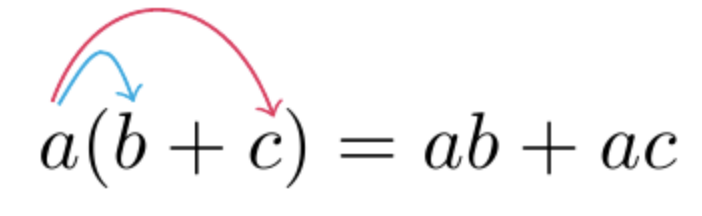
\includegraphics[width=5cm]{pics/distributive}
\end{figure*}
% ====== Example 5
\begin{exa}
	Simplify $2(3x-10)$.
\end{exa}
\vspace{-0.4cm}
\begin{align*}
	2(3x-10)& &&\text{Distribute $2$ over $3x$ and $-10$}\\
	2(3x)+2(-10)& &&\text{Multiply}\\
	6x-20&	&&\text{Our solution}
\end{align*}
\vspace{0.4cm}
% ====== Example 6
\begin{exa}
	Simplify $-6(-4+6y)$.
\end{exa}
\begin{align*}
	-6(-4+6y)& &&\text{Distribute $-6$ over $-4$ and $6y$}\\
	-6(-4)-6(6y)& &&\text{Multiply}\\
	24-36y&	&&\text{Our solution}
\end{align*}
% =======
\begin{nt}
	The most common error in distributing is a sign error, be very
careful with your signs!
\end{nt}
% ========
\begin{nt}
	It is possible to distribute just a negative through parenthesis. If we have a negative in front of parenthesis we can think of it like a "$−1$" in front and distribute the "$-1$" through. This is shown in the following example.
\end{nt}
% ====== EXAMPLE 7
\begin{exa}
	Simplify $-(7y-4x+z-3)$.
\end{exa}
\begin{align*}
	-1(7y-4x+z-3)& &&\text{Negative can be thought of as $-1$}\\
	-1(7y)-1(-4x)-1(z)-1(-3)& &&\text{Multiply each term by $-1$}\\
	-7y+4x-z+3&	&&\text{Our solution}
\end{align*}
% ====== EXAMPLE 8
\begin{exa}
	Simplify $5+2(3x-8)$.
\end{exa}
\begin{align*}
	5+2(3x-8)& &&\text{Distribute 2, multiply each term by 2}\\
	5+6x-16& &&\text{Combine like terms}\\
	6x-11&	&&\text{Our solution}
\end{align*}
% ===== EXAMPLE 9
\begin{exa}
	Simplify $4(6x-1)-(4x-19)$.
\end{exa}
\vspace{-0.4cm}
\begin{align*}
	4(6x-1)-(4x-19)& 
	&&\text{Negative in middle can be thought of as $− 1$}\\
	4(6x-1)-1(4x-19)& 
	&&\text{Distribute}\\
	24x-4-4x+19&	&&\text{Combine like terms}\\
	20x+15& &&\text{Our solution}
\end{align*}
% ========
\section{Absolute Value}
The absolute value of a real number a is denoted by $|a|$. it is the distance from a to the origin 0 on the number line. For example, the $\left|\,3\,\right|$ is a distance from 3 to 0, which is 3.
\begin{center}
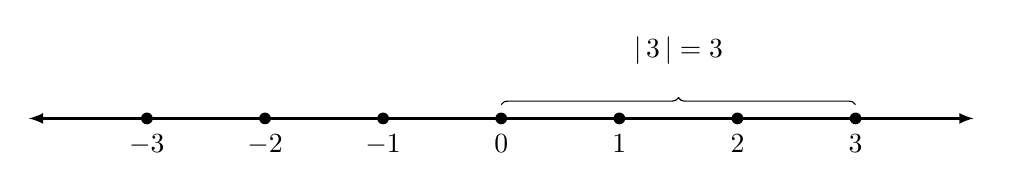
\begin{tikzpicture}[xscale=1.5]
    \draw[thick,latex-latex] (-4,0) -- (4,0)node[right]{};
    \foreach \x in {-3,-2,-1,0,1,2,3}{
    \node[fill,circle,inner sep=1.5pt,label=below:$\x$] at (\x,0) {};
        };
    \draw[decoration={brace,raise=5pt},decorate]
  (0,0) -- node[right=6pt] {} (3,0);
  \node[inner sep=1.5pt,label={above:$|\,3\,|=3$}] at (1.5,0.5) {};
\end{tikzpicture}
\end{center}
%
Another example is $|-2|$.The distance from $-2$ to 0 is $+2$.
%
\begin{center}
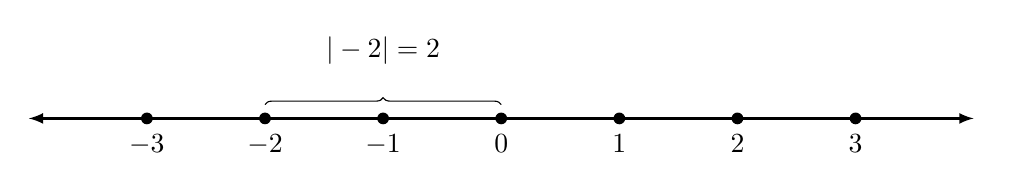
\begin{tikzpicture}[xscale=1.5]
    \draw[thick,latex-latex] (-4,0) -- (4,0)node[right]{};
    \foreach \x in {-3,-2,-1,0,1,2,3}{
    \node[fill,circle,inner sep=1.5pt,label=below:$\x$] at (\x,0) {};
        };
    \draw[decoration={brace,raise=5pt},decorate]
  (-2,0) -- node[right=6pt] {} (0,0);
  \node[inner sep=1.5pt,label={above:$|-2|=2$}] at (-1,0.5) {};
\end{tikzpicture}
\end{center}
%
As you can see, because the absolute value represent a distance, therefore it is always positive. 


\begin{align*}
        	\bigl|number\bigr| = \circled{+}
\end{align*}


We can give a formula for the absolute value of
the number, which depends on whether a is positive or negative.
\begin{empheq}[left={|\,a\,|= \empheqlbrace}]{align*}
    a& \quad \text{if a is positive} \\
    -a& \quad \text{if a is negative}
\end{empheq}
% ====== Example 10
\begin{exa}
    Evaluate $4-|-4-5|$.
\end{exa}
Begin by evaluating inside the absolute value:
\begin{align*}
    4-|-4-5|&   &&\text{$-4-5$ is equal to $-9$}\\
    4-|-9|&     &&\text{The absolute value of $-9$ is 9}\\
    4-(9)&      &&\text{Subtract}\\
    -5&         &&\text{Our solution}
\end{align*}
\subsection{Properties of absolute value}
Some additional useful properties are given below. 
\begin{tcolorbox}[  
                    colback=blue!5!white,
                    ,colframe=blue!75!red, 
                     sharp corners=all
                    ]
    \begin{itemize}
        \item $|\,a\,|\ge 0$,\quad Non-negativity
        \item $|\,a\,|=0 \Longleftrightarrow a=0$,\quad 	Positive-definiteness
        \item $|\,a\,|=|-a|$,\quad 	Evenness
        \item $|\,ab\,|=|a|\,|b|$,\quad Multiplicative
        \item $\displaystyle \biggl|\,\frac{a}{b}\,\biggr|=\frac{|\,a\,|}{|\,b\,|}$,\quad Preservation of division 
    \end{itemize}
\end{tcolorbox}
\subsection{Absolute value equations}
When solving equations with absolute value we can end up with more than one
possible answer. This is because what is in the absolute value can be either negative
or positive and we must account for both possibilities when solving equations.
% ======== example 11
\begin{exa}
    Solve $|x|=4$
\end{exa}
Absolute value can be positive and negative, so our solution is\[
        x=4\ \ or\ \ x=-7
\]
\begin{nt}
When we have absolute values in our problem it is important to first isolate the absolute value, then remove the absolute value by considering both the positive and negative solutions.
\end{nt}
% ====== Example 12
\begin{exa}
    Solve $7+|x|=10$
\end{exa}
Notice that absolute value is not alone. 
\begin{align*}
     7+|x| & = 10 &&\text{Subtract 7 from both sides} \\
    |x|&=3 &&\\
    x=3\quad or&\quad x=-3 &&\text{Our answers}
\end{align*}
The following example requires two steps to isolate the absolute
value. The idea is the same as a two-step equation, add or subtract, then multiply or divide.
%===== Example 13
\begin{exa}
    Solve $-6|x|+2=-10$
\end{exa}
\begin{align*}
    -6|x|+2 &= -10  &&\text{Isolate $|x|$, Subtract 2 from both sides}\\
    -6|x| &= -12    &&\text{Divide both sides by -6}\\
    |x| & =2        &&\text{Absolute value can be positive or negative}\\
    x=2&\quad   or \quad    x=-2    &&\text{Our solution}
\end{align*}
